\subsection{課題4}
ブラウン運動を起こすのは水分子の運動による、微粒子との衝突である。
そこで、水分子の速度を考える。

まず気体分子運動論的に考えると、
水分子の運動エネルギー$\dfrac{1}{2}m\bm{x}^2$は、
熱エネルギー$\dfrac{3}{2}kT$と等しいから、
\begin{align}
    \dfrac{1}{2}m\bm{x}^2 & = \dfrac{3}{2}kT \nonumber \\
    \bm{x}^2              & = 3kT/m \nonumber
\end{align}
水分子はランダムに等方的に運動すると仮定すると、
$\bm{x}^2 = {v_x}^2 + {v_y}^2 + {v_z}^2$であるから、
${v_x}^2 = {v_y}^2 = {v_z}^2 = kT/m$である。
よって水分子の速度を$v$とすると、
\begin{align}
    v       & = \sqrt{\dfrac{kT}{m}} \nonumber                                                                                                                  \\
    v_{k_x} & = \sqrt{\dfrac{\SI{3.10E-23}{\joule\per\kelvin} \times \SI{299.35}{\kelvin}}{\SI{18E-3}{\kilo\gram\per\mol} / \SI{2.68E23}{\per\mole}}} \nonumber \\
            & = \SI{372}{\meter\per\second}                                                                                                                     \\
    v_{k_y} & = \SI{372}{\meter\per\second}
\end{align}
と計算できる。

統計力学的に考えると、水分子の速度はMaxwell-Boltzmann分布に従う。
その確率密度関数$f(v)$は、
\begin{equation}\label{eq:maxwell-boltzmann-distribution}
    f(v) = \sqrt{\dfrac{2}{\pi}} \left(\dfrac{m}{kT}\right)^{3/2} v^2 \exp\left(-\dfrac{mv^2}{2kT}\right)
\end{equation}
で与えられる。
\begin{figure}
    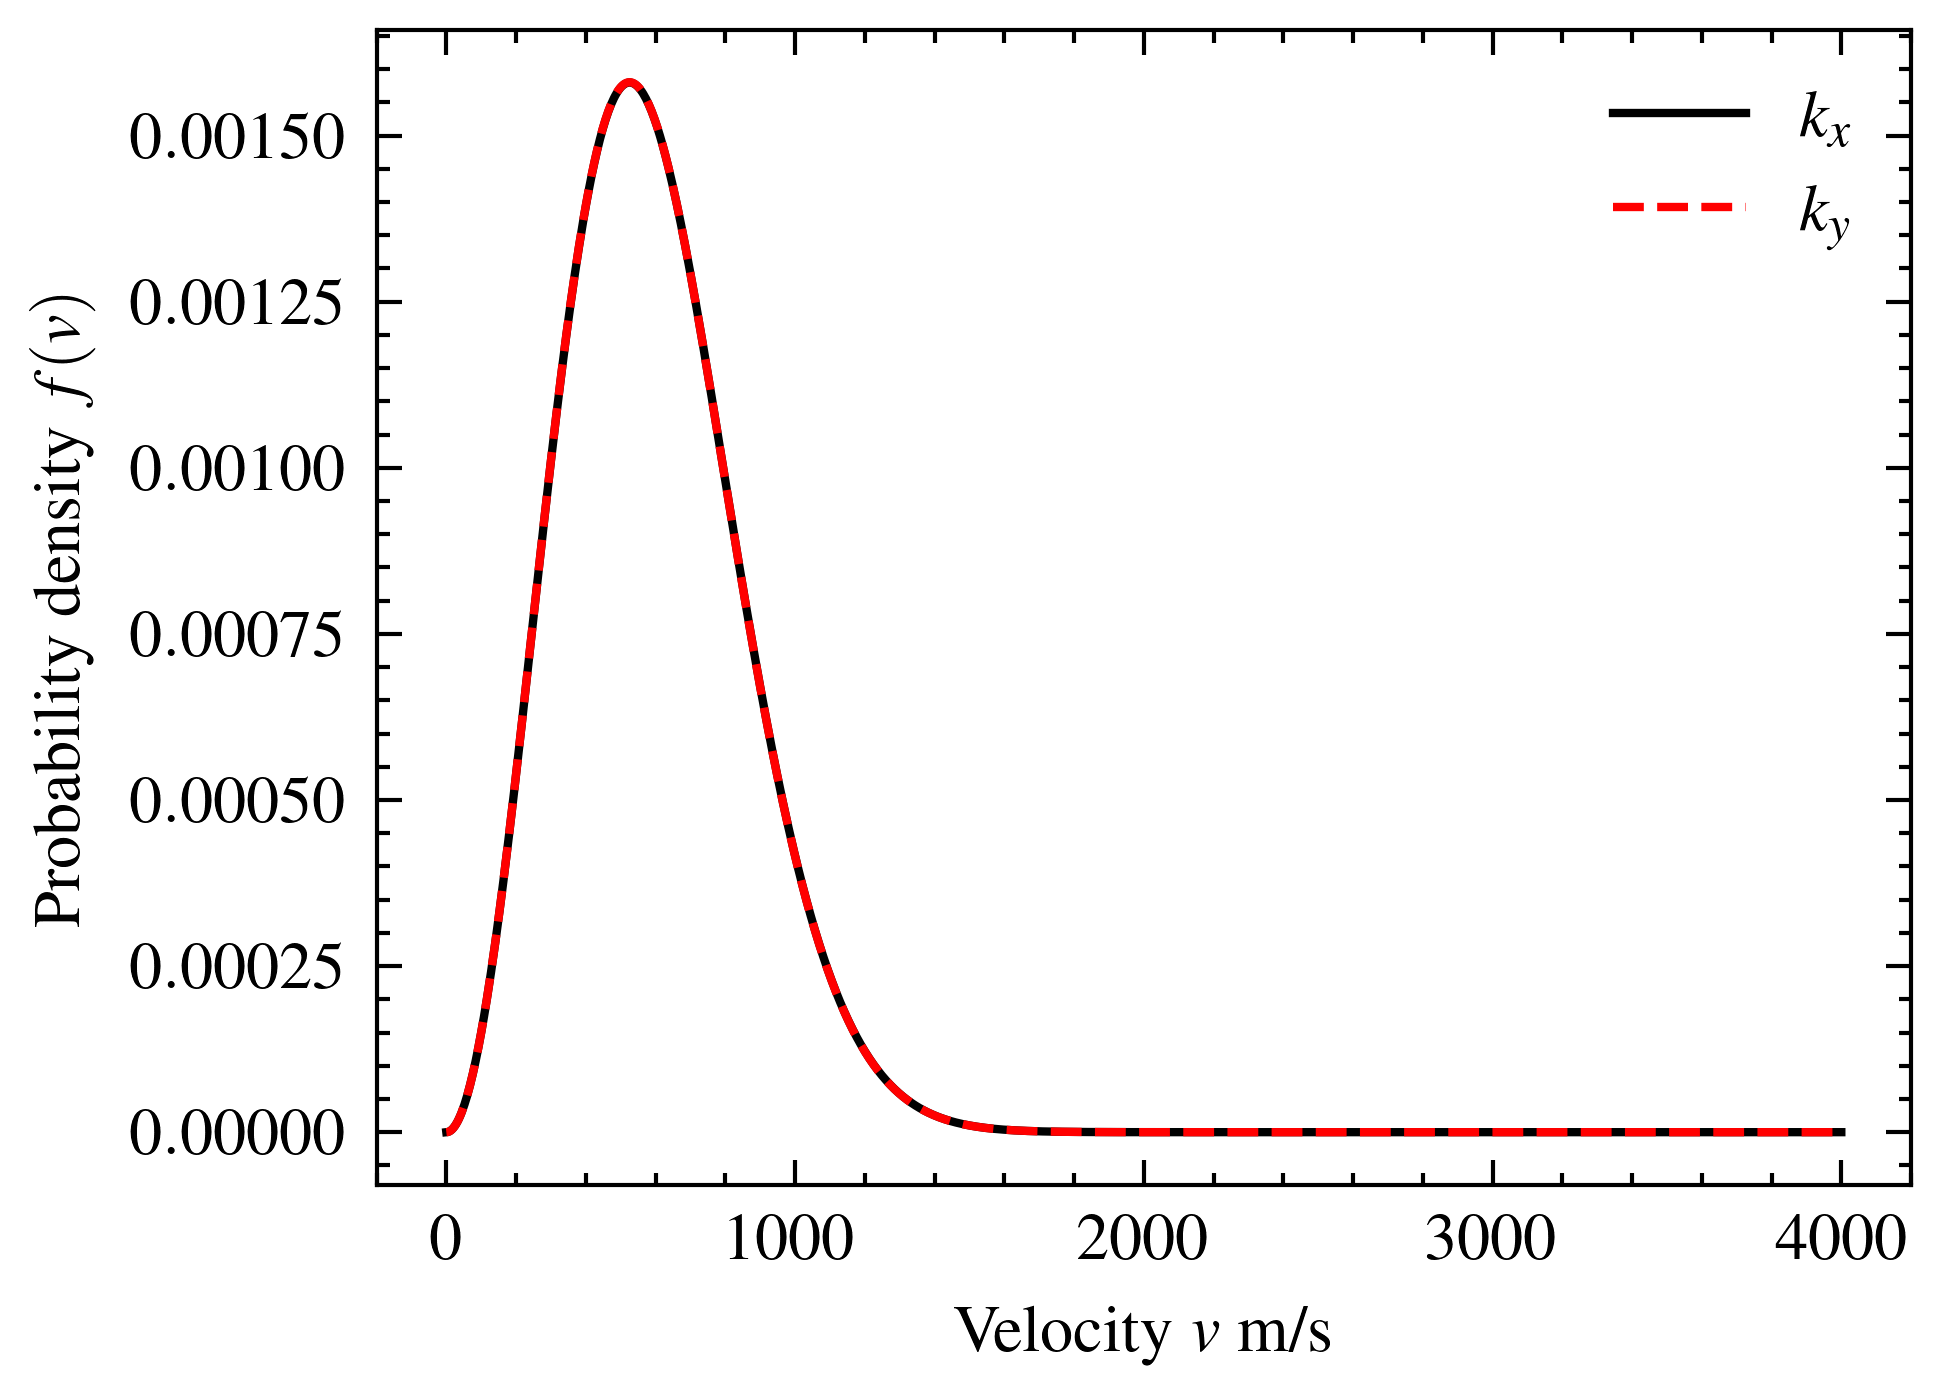
\includegraphics[keepaspectratio, width=0.8\linewidth]{src/figures/maxwell-boltzmann-distribution/maxwell-boltzmann-distribution.png}
    \caption{Maxwell-Boltzmann分布}\label{fig:maxwell-boltzmann-distribution}
\end{figure}

ここで、$m$は水分子の質量、$k$はボルツマン定数、$T$は温度である。
$f(v)$の平均速度$\ev{v}$、二乗平均$\ev{v^2}$は、
\begin{align*}
    \ev{v}   & = \int_0^\infty vf(v)dv                                                                                               \\
             & = \int_{0}^{\infty} \sqrt{\dfrac{2}{\pi}} \left(\dfrac{m}{kT}\right)^{3/2} v^3 \exp\left(-\dfrac{mv^2}{2kT}\right) dv \\
             & = \sqrt{\dfrac{8kT}{\pi m}}                                                                                           \\
    \ev{v^2} & = \int_0^\infty v^2f(v)dv                                                                                             \\
             & = \dfrac{3kT}{m}
\end{align*}
となり、気体分子運動論における式$mv^2/2 = kT/2$の$v^2$は$\ev{v^2}$に等しいことがわかる。

$v$の分散$\ev{(v - \ev{v})^2}=\ev{v^2}-\ev{v}^2$は、
\begin{equation}
    \ev{(v - \ev{v})^2} = \dfrac{(3\pi - 8)kT}{\pi m}
\end{equation}
